% Diagrama de arquitectura de Noticias Verificadas.
% Se compila aparte (pdflatex arquitectura.tex) y el informe incluye el PDF.
\documentclass[tikz,border=6pt]{standalone}
\usepackage[utf8]{inputenc}
\usepackage[T1]{fontenc}
\usepackage{lmodern}
\usetikzlibrary{positioning,arrows.meta,fit,backgrounds}

\definecolor{azulUVG}{RGB}{30,90,150}
\definecolor{verde}{RGB}{46,139,87}
\definecolor{grisclaro}{RGB}{240,243,246}
\definecolor{gristexto}{RGB}{90,100,110}
\definecolor{naranja}{RGB}{184,78,8}

\begin{document}
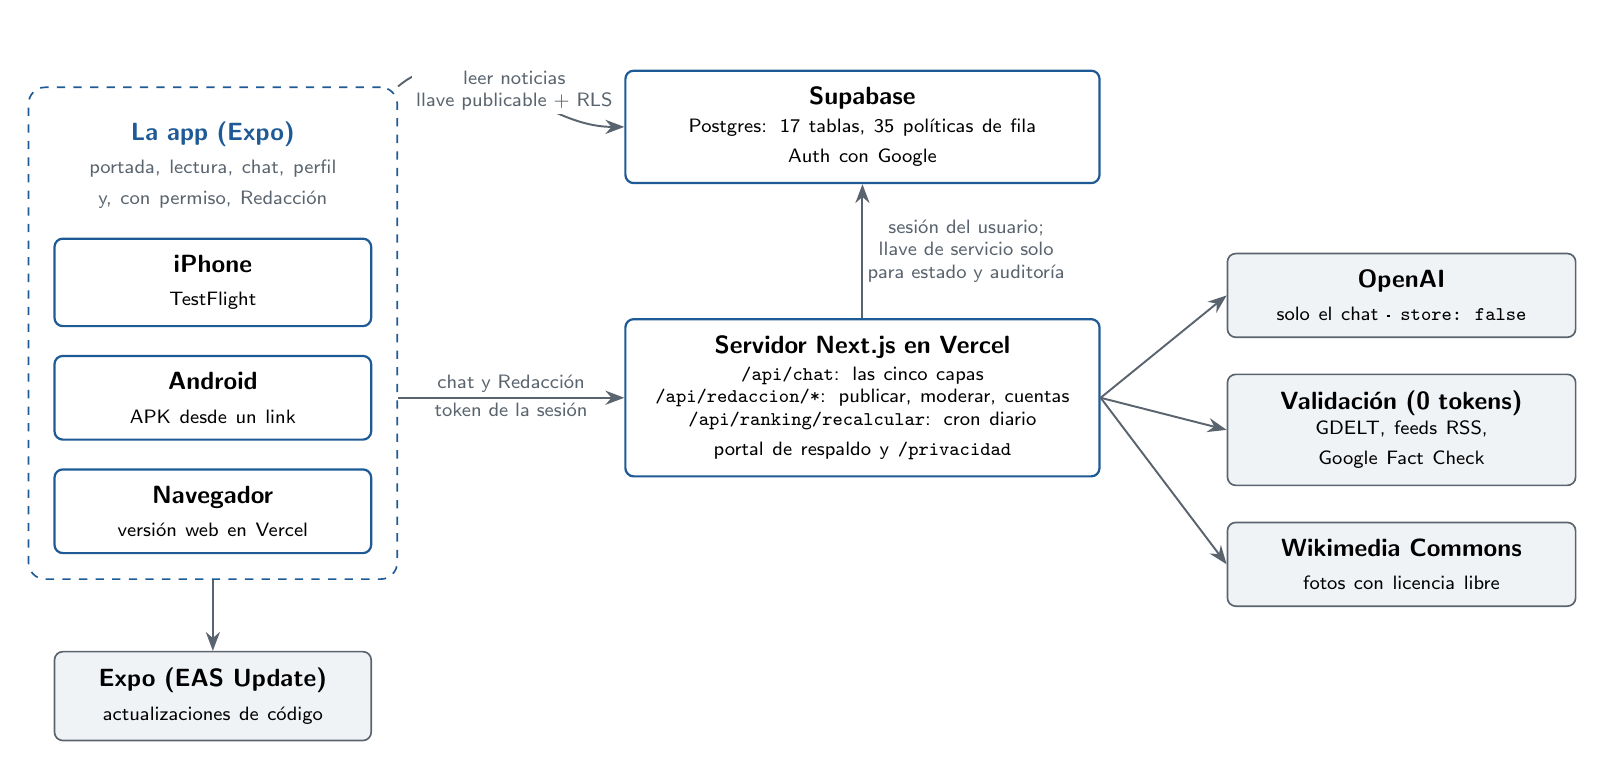
\begin{tikzpicture}[
  font=\sffamily\small,
  caja/.style={draw=azulUVG, line width=0.8pt, rounded corners=3pt, fill=white,
               align=center, inner sep=6pt, text width=#1},
  caja/.default=4.2cm,
  externo/.style={draw=gristexto, line width=0.6pt, rounded corners=3pt, fill=grisclaro,
                  align=center, inner sep=6pt, text width=#1},
  externo/.default=4.2cm,
  flecha/.style={-{Stealth[length=2.4mm]}, line width=0.7pt, color=gristexto},
  rotulo/.style={font=\sffamily\scriptsize, color=gristexto, align=center, fill=white, inner sep=1.5pt},
  grupo/.style={draw=#1, dashed, rounded corners=6pt, inner sep=9pt, line width=0.6pt},
]

% ----- Dispositivos -----
\node[caja=3.6cm] (ios) {\textbf{iPhone}\\[1pt]{\scriptsize TestFlight}};
\node[caja=3.6cm, below=0.35cm of ios] (android) {\textbf{Android}\\[1pt]{\scriptsize APK desde un link}};
\node[caja=3.6cm, below=0.35cm of android] (web) {\textbf{Navegador}\\[1pt]{\scriptsize versión web en Vercel}};
\node[font=\sffamily\small, color=azulUVG, above=0.25cm of ios, align=center, text width=3.8cm] (tituloapp)
  {\textbf{La app (Expo)}\\[1pt]{\scriptsize\color{gristexto} portada, lectura, chat, perfil y, con permiso, Redacción}};
\begin{scope}[on background layer]
  \node[grupo=azulUVG, fit=(tituloapp)(ios)(android)(web)] (app) {};
\end{scope}

% ----- Servidor -----
\node[caja=5.6cm, right=3.2cm of android] (servidor) {%
  \textbf{Servidor Next.js en Vercel}\\[2pt]
  {\scriptsize \texttt{/api/chat}: las cinco capas\\
   \texttt{/api/redaccion/*}: publicar, moderar, cuentas\\
   \texttt{/api/ranking/recalcular}: cron diario\\
   portal de respaldo y \texttt{/privacidad}}};

% ----- Supabase -----
\node[caja=5.6cm, above=1.7cm of servidor] (supabase) {%
  \textbf{Supabase}\\[2pt]
  {\scriptsize Postgres: 17 tablas, 35 políticas de fila\\
   Auth con Google}};

% ----- Externos -----
\node[externo=4.0cm, right=1.6cm of servidor, yshift=1.3cm] (openai) {%
  \textbf{OpenAI}\\[1pt]{\scriptsize solo el chat · \texttt{store: false}}};
\node[externo=4.0cm, below=0.45cm of openai] (validacion) {%
  \textbf{Validación (0 tokens)}\\[1pt]{\scriptsize GDELT, feeds RSS,\\ Google Fact Check}};
\node[externo=4.0cm, below=0.45cm of validacion] (commons) {%
  \textbf{Wikimedia Commons}\\[1pt]{\scriptsize fotos con licencia libre}};
\node[externo=3.6cm, below=0.9cm of app] (expo) {%
  \textbf{Expo (EAS Update)}\\[1pt]{\scriptsize actualizaciones de código}};

% ----- Flechas -----
\draw[flecha] (app.north east) to[out=40,in=180]
  node[rotulo, pos=0.55] {leer noticias\\llave publicable + RLS} (supabase.west);
\draw[flecha] (app.east |- servidor.west) -- node[rotulo, above] {chat y Redacción}
  node[rotulo, below] {token de la sesión} (servidor.west);
\draw[flecha] (servidor.north) -- node[rotulo, right] {sesión del usuario;\\llave de servicio solo\\para estado y auditoría} (supabase.south);
\draw[flecha] (servidor.east) -- (openai.west);
\draw[flecha] (servidor.east) -- (validacion.west);
\draw[flecha] (servidor.east) -- (commons.west);
\draw[flecha] (app.south) -- (expo.north);

\end{tikzpicture}
\end{document}
